\documentclass{book}
\usepackage[a4paper,top=2.5cm,bottom=2.5cm,left=2.5cm,right=2.5cm]{geometry}
\usepackage{makeidx}
\usepackage{natbib}
\usepackage{graphicx}
\usepackage{multicol}
\usepackage{float}
\usepackage{listings}
\usepackage{color}
\usepackage{ifthen}
\usepackage[table]{xcolor}
\usepackage{textcomp}
\usepackage{alltt}
\usepackage{ifpdf}
\ifpdf
\usepackage[pdftex,
            pagebackref=true,
            colorlinks=true,
            linkcolor=blue,
            unicode
           ]{hyperref}
\else
\usepackage[ps2pdf,
            pagebackref=true,
            colorlinks=true,
            linkcolor=blue,
            unicode
           ]{hyperref}
\usepackage{pspicture}
\fi
\usepackage[utf8]{inputenc}
\usepackage[french]{babel}

\usepackage{mathptmx}
\usepackage[scaled=.90]{helvet}
\usepackage{courier}
\usepackage{sectsty}
\usepackage{amssymb}
\usepackage[titles]{tocloft}
\usepackage{doxygen}
\lstset{language=C++,inputencoding=utf8,basicstyle=\footnotesize,breaklines=true,breakatwhitespace=true,tabsize=8,numbers=left }
\makeindex
\setcounter{tocdepth}{3}
\renewcommand{\footrulewidth}{0.4pt}
\renewcommand{\familydefault}{\sfdefault}
\hfuzz=15pt
\setlength{\emergencystretch}{15pt}
\hbadness=750
\tolerance=750
\begin{document}
\hypersetup{pageanchor=false,citecolor=blue}
\begin{titlepage}
\vspace*{7cm}
\begin{center}
{\Large Organizer }\\
\vspace*{1cm}
{\large Généré par Doxygen 1.8.1.2}\\
\vspace*{0.5cm}
{\small Mardi Janvier 14 2014 17:35:43}\\
\end{center}
\end{titlepage}
\clearemptydoublepage
\pagenumbering{roman}
\tableofcontents
\clearemptydoublepage
\pagenumbering{arabic}
\hypersetup{pageanchor=true,citecolor=blue}
\chapter{Index des classes}
\section{Hiérarchie des classes}
Cette liste d'héritage est classée approximativement par ordre alphabétique \-:\begin{DoxyCompactList}
\item \contentsline{section}{Doublon}{\pageref{class_doublon}}{}
\item \contentsline{section}{Doublon\-Model}{\pageref{class_doublon_model}}{}
\item \contentsline{section}{Doublon\-Tree}{\pageref{class_doublon_tree}}{}
\item \contentsline{section}{M\-D5\-Key}{\pageref{class_m_d5_key}}{}
\item \contentsline{section}{Organizer}{\pageref{class_organizer}}{}
\begin{DoxyCompactList}
\item \contentsline{section}{Org\-View}{\pageref{class_org_view}}{}
\end{DoxyCompactList}
\item \contentsline{section}{Ui\-\_\-\-Org\-View}{\pageref{class_ui___org_view}}{}
\begin{DoxyCompactList}
\item \contentsline{section}{Ui\-:\-:Org\-View}{\pageref{class_ui_1_1_org_view}}{}
\end{DoxyCompactList}
\end{DoxyCompactList}

\chapter{Index des classes}
\section{Liste des classes}
Liste des classes, structures, unions et interfaces avec une brève description \-:\begin{DoxyCompactList}
\item\contentsline{section}{{\bf Doublon} \\*Classe représentant le \doxyref{Doublon}{p.}{class_doublon} }{\pageref{class_doublon}}{}
\item\contentsline{section}{{\bf Doublon\-Model} \\*La classe \doxyref{Doublon\-Model}{p.}{class_doublon_model} permettant la représentation en arbre d'une liste de doubons }{\pageref{class_doublon_model}}{}
\item\contentsline{section}{{\bf Doublon\-Tree} \\*La classe \doxyref{Doublon\-Tree}{p.}{class_doublon_tree} }{\pageref{class_doublon_tree}}{}
\item\contentsline{section}{{\bf M\-D5\-Key} \\*Classe représentant la clé M\-D5 }{\pageref{class_m_d5_key}}{}
\item\contentsline{section}{{\bf Organizer} \\*Classe représentant l'application }{\pageref{class_organizer}}{}
\item\contentsline{section}{{\bf Ui\-::\-Org\-View} }{\pageref{class_ui_1_1_org_view}}{}
\item\contentsline{section}{{\bf Org\-View} \\*Classe représentant l'affichage de l'application }{\pageref{class_org_view}}{}
\item\contentsline{section}{{\bf Ui\-\_\-\-Org\-View} }{\pageref{class_ui___org_view}}{}
\end{DoxyCompactList}

\chapter{Index des fichiers}
\section{Liste des fichiers}
Liste de tous les fichiers documentés avec une brève description \-:\begin{DoxyCompactList}
\item\contentsline{section}{{\bf doublon.\-cpp} \\*Définit les doublons }{\pageref{doublon_8cpp}}{}
\item\contentsline{section}{{\bf doublon.\-h} \\*Définit les doublons }{\pageref{doublon_8h}}{}
\item\contentsline{section}{{\bf doublonmodel.\-h} \\*Définit le modèle représentant les doublons }{\pageref{doublonmodel_8h}}{}
\item\contentsline{section}{{\bf doublontree.\-cpp} \\*Définit la structure d'un noeud de l'arbre de doublons }{\pageref{doublontree_8cpp}}{}
\item\contentsline{section}{{\bf doublontree.\-h} \\*Définit la structure d'un noeud de l'arbre de doublons }{\pageref{doublontree_8h}}{}
\item\contentsline{section}{{\bf md5key.\-h} \\*Définit les clé M\-D5 des doublons }{\pageref{md5key_8h}}{}
\item\contentsline{section}{{\bf organizer.\-h} \\*Définit les méthodes de l'application }{\pageref{organizer_8h}}{}
\item\contentsline{section}{{\bf orgview.\-h} \\*Définit l'afichage de l'application }{\pageref{orgview_8h}}{}
\item\contentsline{section}{{\bfseries ui\-\_\-orgview.\-h} }{\pageref{ui__orgview_8h}}{}
\end{DoxyCompactList}

\chapter{Documentation des classes}
\section{Référence de la classe Doublon}
\label{class_doublon}\index{Doublon@{Doublon}}


Classe représentant le \doxyref{Doublon}{p.}{class_doublon}.  




{\ttfamily \#include $<$doublon.\-h$>$}

\subsection*{Fonctions membres publiques}
\begin{DoxyCompactItemize}
\item 
{\bf Doublon} (const std\-::string \&path)
\begin{DoxyCompactList}\small\item\em Constructeur de la classe \doxyref{Doublon}{p.}{class_doublon}. \end{DoxyCompactList}\item 
void {\bf set\-Key} (const unsigned char $\ast$md5)
\begin{DoxyCompactList}\small\item\em Setteur de la clé M\-D5. \end{DoxyCompactList}\item 
{\bf M\-D5\-Key} $\ast$ {\bf get\-Key} () const 
\begin{DoxyCompactList}\small\item\em Getteur de la clé M\-D5. \end{DoxyCompactList}\item 
const char $\ast$ {\bf get\-Path} () const 
\begin{DoxyCompactList}\small\item\em Getteur du chemin du fichier. \end{DoxyCompactList}\item 
{\bf $\sim$\-Doublon} ()\label{class_doublon_a67ab3ff0d90f6eaccd061a12c07ad14b}

\begin{DoxyCompactList}\small\item\em Destructeur de la classe \doxyref{Doublon}{p.}{class_doublon}. \end{DoxyCompactList}\end{DoxyCompactItemize}


\subsection{Description détaillée}
Classe représentant le \doxyref{Doublon}{p.}{class_doublon}. 

\subsection{Documentation des constructeurs et destructeur}
\index{Doublon@{Doublon}!Doublon@{Doublon}}
\index{Doublon@{Doublon}!Doublon@{Doublon}}
\subsubsection[{Doublon}]{\setlength{\rightskip}{0pt plus 5cm}Doublon\-::\-Doublon (
\begin{DoxyParamCaption}
\item[{const std\-::string \&}]{path}
\end{DoxyParamCaption}
)}\label{class_doublon_ad1f964eed7fce399af6ea6452fe893ba}


Constructeur de la classe \doxyref{Doublon}{p.}{class_doublon}. 


\begin{DoxyParams}[1]{Paramètres}
\mbox{\tt in}  & {\em path} & \-: chemin absolu du fichier \\
\hline
\end{DoxyParams}


\subsection{Documentation des fonctions membres}
\index{Doublon@{Doublon}!get\-Key@{get\-Key}}
\index{get\-Key@{get\-Key}!Doublon@{Doublon}}
\subsubsection[{get\-Key}]{\setlength{\rightskip}{0pt plus 5cm}{\bf M\-D5\-Key}$\ast$ Doublon\-::get\-Key (
\begin{DoxyParamCaption}
{}
\end{DoxyParamCaption}
) const\hspace{0.3cm}{\ttfamily [inline]}}\label{class_doublon_acb10240d73107451307058c4be69edd5}


Getteur de la clé M\-D5. 

\begin{DoxyReturn}{Renvoie}
Pointeur sur l'objet représentant la clé M\-D5 
\end{DoxyReturn}
\index{Doublon@{Doublon}!get\-Path@{get\-Path}}
\index{get\-Path@{get\-Path}!Doublon@{Doublon}}
\subsubsection[{get\-Path}]{\setlength{\rightskip}{0pt plus 5cm}const char$\ast$ Doublon\-::get\-Path (
\begin{DoxyParamCaption}
{}
\end{DoxyParamCaption}
) const\hspace{0.3cm}{\ttfamily [inline]}}\label{class_doublon_a2f915aec59153d41cbc8fc877249ff3c}


Getteur du chemin du fichier. 

\begin{DoxyReturn}{Renvoie}
Pointeur sur le tableau contenant le chemin du fichier 
\end{DoxyReturn}
\index{Doublon@{Doublon}!set\-Key@{set\-Key}}
\index{set\-Key@{set\-Key}!Doublon@{Doublon}}
\subsubsection[{set\-Key}]{\setlength{\rightskip}{0pt plus 5cm}void Doublon\-::set\-Key (
\begin{DoxyParamCaption}
\item[{const unsigned char $\ast$}]{md5}
\end{DoxyParamCaption}
)\hspace{0.3cm}{\ttfamily [inline]}}\label{class_doublon_a7fcfdaf97e53756e128d5af00a997d85}


Setteur de la clé M\-D5. 


\begin{DoxyParams}[1]{Paramètres}
\mbox{\tt in}  & {\em md5} & \-: tableau correspondant à la clé M\-D5 du fichier \\
\hline
\end{DoxyParams}


La documentation de cette classe a été générée à partir des fichiers suivants \-:\begin{DoxyCompactItemize}
\item 
{\bf doublon.\-h}\item 
{\bf doublon.\-cpp}\end{DoxyCompactItemize}

\hypertarget{class_doublon_model}{\section{Référence de la classe Doublon\-Model}
\label{class_doublon_model}\index{Doublon\-Model@{Doublon\-Model}}
}
\subsection*{Fonctions membres publiques}
\begin{DoxyCompactItemize}
\item 
\hypertarget{class_doublon_model_a33c5fb7b1b039ca333453024f461afdd}{{\bfseries Doublon\-Model} (const Q\-String \&data, Q\-Object $\ast$parent=0)}\label{class_doublon_model_a33c5fb7b1b039ca333453024f461afdd}

\item 
\hypertarget{class_doublon_model_a10e14770aec49a113eb478af1c869bbb}{Q\-Variant {\bfseries data} (const Q\-Model\-Index \&index, int role) const }\label{class_doublon_model_a10e14770aec49a113eb478af1c869bbb}

\item 
\hypertarget{class_doublon_model_aff5724d094400fd653e4d35ab4a2bfea}{Qt\-::\-Item\-Flags {\bfseries flags} (const Q\-Model\-Index \&index) const }\label{class_doublon_model_aff5724d094400fd653e4d35ab4a2bfea}

\item 
\hypertarget{class_doublon_model_aafaab9974fb6f13dfed5b352051a9c8b}{Q\-Variant {\bfseries header\-Data} (int section, Qt\-::\-Orientation orientation, int role=Qt\-::\-Display\-Role) const }\label{class_doublon_model_aafaab9974fb6f13dfed5b352051a9c8b}

\item 
\hypertarget{class_doublon_model_a43711f335c10c2d82cba2ba935d5d903}{Q\-Model\-Index {\bfseries index} (int row, int column, const Q\-Model\-Index \&parent=Q\-Model\-Index()) const }\label{class_doublon_model_a43711f335c10c2d82cba2ba935d5d903}

\item 
\hypertarget{class_doublon_model_a4b63ebbfb27fe9bbe52647f175d72d39}{Q\-Model\-Index {\bfseries parent} (const Q\-Model\-Index \&index) const }\label{class_doublon_model_a4b63ebbfb27fe9bbe52647f175d72d39}

\item 
\hypertarget{class_doublon_model_a387f51df68f693ea20af3ab968ca4df6}{int {\bfseries row\-Count} (const Q\-Model\-Index \&parent=Q\-Model\-Index()) const }\label{class_doublon_model_a387f51df68f693ea20af3ab968ca4df6}

\item 
\hypertarget{class_doublon_model_a47458991a1f0e7f4ae8bf79af4ff0c16}{int {\bfseries column\-Count} (const Q\-Model\-Index \&parent=Q\-Model\-Index()) const }\label{class_doublon_model_a47458991a1f0e7f4ae8bf79af4ff0c16}

\item 
\hypertarget{class_doublon_model_a3188f8b049e9da84ca293b8e62990ba3}{void {\bfseries setup\-Model\-Data} (const Q\-String \&line, const u\-\_\-int8\-\_\-t type, \hyperlink{class_doublon_tree}{Doublon\-Tree} $\ast$parent)}\label{class_doublon_model_a3188f8b049e9da84ca293b8e62990ba3}

\end{DoxyCompactItemize}
\subsection*{Attributs publics}
\begin{DoxyCompactItemize}
\item 
\hypertarget{class_doublon_model_ad622e10652206f0f725b2aec69d11a18}{\hyperlink{class_doublon_tree}{Doublon\-Tree} $\ast$ {\bfseries root\-Item}}\label{class_doublon_model_ad622e10652206f0f725b2aec69d11a18}

\end{DoxyCompactItemize}


La documentation de cette classe a été générée à partir des fichiers suivants \-:\begin{DoxyCompactItemize}
\item 
doublonmodel.\-h\item 
doublonmodel.\-cpp\end{DoxyCompactItemize}

\hypertarget{class_doublon_tree}{\section{Référence de la classe Doublon\-Tree}
\label{class_doublon_tree}\index{Doublon\-Tree@{Doublon\-Tree}}
}
\subsection*{Fonctions membres publiques}
\begin{DoxyCompactItemize}
\item 
\hypertarget{class_doublon_tree_aeef7a22a4ecbbd4e936325c9699848a0}{{\bfseries Doublon\-Tree} (const Q\-Variant \&data, const u\-\_\-int8\-\_\-t type, \hyperlink{class_doublon_tree}{Doublon\-Tree} $\ast$parent=0)}\label{class_doublon_tree_aeef7a22a4ecbbd4e936325c9699848a0}

\item 
\hypertarget{class_doublon_tree_aa6b40c180f310fcd948fb2629b2ef10c}{void {\bfseries append\-Child} (\hyperlink{class_doublon_tree}{Doublon\-Tree} $\ast$child)}\label{class_doublon_tree_aa6b40c180f310fcd948fb2629b2ef10c}

\item 
\hypertarget{class_doublon_tree_a03b05097f7c811686d7a7ae67f56b8ee}{\hyperlink{class_doublon_tree}{Doublon\-Tree} $\ast$ {\bfseries child} (int row)}\label{class_doublon_tree_a03b05097f7c811686d7a7ae67f56b8ee}

\item 
\hypertarget{class_doublon_tree_ad048f4249d32acc81a203465f5569312}{int {\bfseries child\-Count} () const }\label{class_doublon_tree_ad048f4249d32acc81a203465f5569312}

\item 
\hypertarget{class_doublon_tree_a587ca20a3be3ed2829b36dbfda00be05}{Q\-Variant {\bfseries data} () const }\label{class_doublon_tree_a587ca20a3be3ed2829b36dbfda00be05}

\item 
\hypertarget{class_doublon_tree_a1ccd8565e780ff0cc31b3b5d982737c0}{int {\bfseries column\-Count} () const }\label{class_doublon_tree_a1ccd8565e780ff0cc31b3b5d982737c0}

\item 
\hypertarget{class_doublon_tree_a108bb7946eef6efb9057911cf90f6095}{int {\bfseries row} () const }\label{class_doublon_tree_a108bb7946eef6efb9057911cf90f6095}

\item 
\hypertarget{class_doublon_tree_a378ba45c738cbebf3e7527b98b457f65}{\hyperlink{class_doublon_tree}{Doublon\-Tree} $\ast$ {\bfseries parent} ()}\label{class_doublon_tree_a378ba45c738cbebf3e7527b98b457f65}

\item 
\hypertarget{class_doublon_tree_a2885ec60d59853eef0b1932f0068e9ca}{u\-\_\-int8\-\_\-t {\bfseries get\-Type} ()}\label{class_doublon_tree_a2885ec60d59853eef0b1932f0068e9ca}

\end{DoxyCompactItemize}


La documentation de cette classe a été générée à partir des fichiers suivants \-:\begin{DoxyCompactItemize}
\item 
doublontree.\-h\item 
doublontree.\-cpp\end{DoxyCompactItemize}

\hypertarget{class_m_d5_key}{\section{Référence de la classe M\-D5\-Key}
\label{class_m_d5_key}\index{M\-D5\-Key@{M\-D5\-Key}}
}


Classe représentant la clé M\-D5.  




{\ttfamily \#include $<$md5key.\-h$>$}

\subsection*{Fonctions membres publiques}
\begin{DoxyCompactItemize}
\item 
\hyperlink{class_m_d5_key_a128484a209773db763f628f2dc8482fc}{M\-D5\-Key} (const unsigned char $\ast$)
\begin{DoxyCompactList}\small\item\em Constructeur de la classe \hyperlink{class_m_d5_key}{M\-D5\-Key}. \end{DoxyCompactList}\item 
const std\-::string \hyperlink{class_m_d5_key_a9f7ce0835cc0d70e316bf8152802c0a8}{to\-String} () const 
\begin{DoxyCompactList}\small\item\em Transforme la clé M\-D5 en string. \end{DoxyCompactList}\end{DoxyCompactItemize}
\subsection*{Amis}
\begin{DoxyCompactItemize}
\item 
bool \hyperlink{class_m_d5_key_ab9ea4f1611018c7e43e9ff0a704dec58}{operator$<$} (const \hyperlink{class_m_d5_key}{M\-D5\-Key} \&k1, const \hyperlink{class_m_d5_key}{M\-D5\-Key} \&k2)
\begin{DoxyCompactList}\small\item\em Surchagre de l'opérateur \char`\"{}inférieur\char`\"{}. \end{DoxyCompactList}\item 
bool \hyperlink{class_m_d5_key_aedad54e0b5f2363c0340a9bb5a62781e}{operator==} (const \hyperlink{class_m_d5_key}{M\-D5\-Key} \&k1, const \hyperlink{class_m_d5_key}{M\-D5\-Key} \&k2)
\begin{DoxyCompactList}\small\item\em Surchagre de l'opérateur \char`\"{}égale\char`\"{}. \end{DoxyCompactList}\item 
bool \hyperlink{class_m_d5_key_a911c35f88bf2d6ba464bb3c62d9b6b69}{operator!=} (const \hyperlink{class_m_d5_key}{M\-D5\-Key} \&k1, const \hyperlink{class_m_d5_key}{M\-D5\-Key} \&k2)
\begin{DoxyCompactList}\small\item\em Surchagre de l'opérateur \char`\"{}inégale\char`\"{}. \end{DoxyCompactList}\end{DoxyCompactItemize}


\subsection{Description détaillée}
Classe représentant la clé M\-D5. 

\subsection{Documentation des constructeurs et destructeur}
\hypertarget{class_m_d5_key_a128484a209773db763f628f2dc8482fc}{\index{M\-D5\-Key@{M\-D5\-Key}!M\-D5\-Key@{M\-D5\-Key}}
\index{M\-D5\-Key@{M\-D5\-Key}!MD5Key@{M\-D5\-Key}}
\subsubsection[{M\-D5\-Key}]{\setlength{\rightskip}{0pt plus 5cm}M\-D5\-Key\-::\-M\-D5\-Key (
\begin{DoxyParamCaption}
\item[{const unsigned char $\ast$}]{md5}
\end{DoxyParamCaption}
)}}\label{class_m_d5_key_a128484a209773db763f628f2dc8482fc}


Constructeur de la classe \hyperlink{class_m_d5_key}{M\-D5\-Key}. 


\begin{DoxyParams}[1]{Paramètres}
\mbox{\tt in}  & {\em path} & \-: chemin aboslu du fichier \\
\hline
\end{DoxyParams}


\subsection{Documentation des fonctions membres}
\hypertarget{class_m_d5_key_a9f7ce0835cc0d70e316bf8152802c0a8}{\index{M\-D5\-Key@{M\-D5\-Key}!to\-String@{to\-String}}
\index{to\-String@{to\-String}!MD5Key@{M\-D5\-Key}}
\subsubsection[{to\-String}]{\setlength{\rightskip}{0pt plus 5cm}const std\-::string M\-D5\-Key\-::to\-String (
\begin{DoxyParamCaption}
{}
\end{DoxyParamCaption}
) const}}\label{class_m_d5_key_a9f7ce0835cc0d70e316bf8152802c0a8}


Transforme la clé M\-D5 en string. 

\begin{DoxyReturn}{Renvoie}
String correspondant à la clé M\-D5 
\end{DoxyReturn}


\subsection{Documentation des fonctions amies et associées}
\hypertarget{class_m_d5_key_a911c35f88bf2d6ba464bb3c62d9b6b69}{\index{M\-D5\-Key@{M\-D5\-Key}!operator!=@{operator!=}}
\index{operator!=@{operator!=}!MD5Key@{M\-D5\-Key}}
\subsubsection[{operator!=}]{\setlength{\rightskip}{0pt plus 5cm}bool operator!= (
\begin{DoxyParamCaption}
\item[{const {\bf M\-D5\-Key} \&}]{k1, }
\item[{const {\bf M\-D5\-Key} \&}]{k2}
\end{DoxyParamCaption}
)\hspace{0.3cm}{\ttfamily [friend]}}}\label{class_m_d5_key_a911c35f88bf2d6ba464bb3c62d9b6b69}


Surchagre de l'opérateur \char`\"{}inégale\char`\"{}. 


\begin{DoxyParams}[1]{Paramètres}
\mbox{\tt in}  & {\em k1} & \-: \hyperlink{class_m_d5_key}{M\-D5\-Key} servant à la comparaison \\
\hline
\mbox{\tt in}  & {\em k2} & \-: \hyperlink{class_m_d5_key}{M\-D5\-Key} servant à la comparaison \\
\hline
\end{DoxyParams}
\begin{DoxyReturn}{Renvoie}
true si l'objet k1 n'est pas égale à l'objet k2 false sinon 
\end{DoxyReturn}
\hypertarget{class_m_d5_key_ab9ea4f1611018c7e43e9ff0a704dec58}{\index{M\-D5\-Key@{M\-D5\-Key}!operator$<$@{operator$<$}}
\index{operator$<$@{operator$<$}!MD5Key@{M\-D5\-Key}}
\subsubsection[{operator$<$}]{\setlength{\rightskip}{0pt plus 5cm}bool operator$<$ (
\begin{DoxyParamCaption}
\item[{const {\bf M\-D5\-Key} \&}]{k1, }
\item[{const {\bf M\-D5\-Key} \&}]{k2}
\end{DoxyParamCaption}
)\hspace{0.3cm}{\ttfamily [friend]}}}\label{class_m_d5_key_ab9ea4f1611018c7e43e9ff0a704dec58}


Surchagre de l'opérateur \char`\"{}inférieur\char`\"{}. 


\begin{DoxyParams}[1]{Paramètres}
\mbox{\tt in}  & {\em k1} & \-: \hyperlink{class_m_d5_key}{M\-D5\-Key} servant à la comparaison \\
\hline
\mbox{\tt in}  & {\em k2} & \-: \hyperlink{class_m_d5_key}{M\-D5\-Key} servant à la comparaison \\
\hline
\end{DoxyParams}
\begin{DoxyReturn}{Renvoie}
true si l'objet k1 est plus petit que l'objet k2 false sinon 
\end{DoxyReturn}
\hypertarget{class_m_d5_key_aedad54e0b5f2363c0340a9bb5a62781e}{\index{M\-D5\-Key@{M\-D5\-Key}!operator==@{operator==}}
\index{operator==@{operator==}!MD5Key@{M\-D5\-Key}}
\subsubsection[{operator==}]{\setlength{\rightskip}{0pt plus 5cm}bool operator== (
\begin{DoxyParamCaption}
\item[{const {\bf M\-D5\-Key} \&}]{k1, }
\item[{const {\bf M\-D5\-Key} \&}]{k2}
\end{DoxyParamCaption}
)\hspace{0.3cm}{\ttfamily [friend]}}}\label{class_m_d5_key_aedad54e0b5f2363c0340a9bb5a62781e}


Surchagre de l'opérateur \char`\"{}égale\char`\"{}. 


\begin{DoxyParams}[1]{Paramètres}
\mbox{\tt in}  & {\em k1} & \-: \hyperlink{class_m_d5_key}{M\-D5\-Key} servant à la comparaison \\
\hline
\mbox{\tt in}  & {\em k2} & \-: \hyperlink{class_m_d5_key}{M\-D5\-Key} servant à la comparaison \\
\hline
\end{DoxyParams}
\begin{DoxyReturn}{Renvoie}
true si l'objet k1 est égale à l'objet k2 false sinon 
\end{DoxyReturn}


La documentation de cette classe a été générée à partir des fichiers suivants \-:\begin{DoxyCompactItemize}
\item 
\hyperlink{md5key_8h}{md5key.\-h}\item 
md5key.\-cpp\end{DoxyCompactItemize}

\section{Référence de la classe Organizer}
\label{class_organizer}\index{Organizer@{Organizer}}


Classe représentant l'application.  




{\ttfamily \#include $<$organizer.\-h$>$}

Graphe d'héritage de Organizer\-:\begin{figure}[H]
\begin{center}
\leavevmode
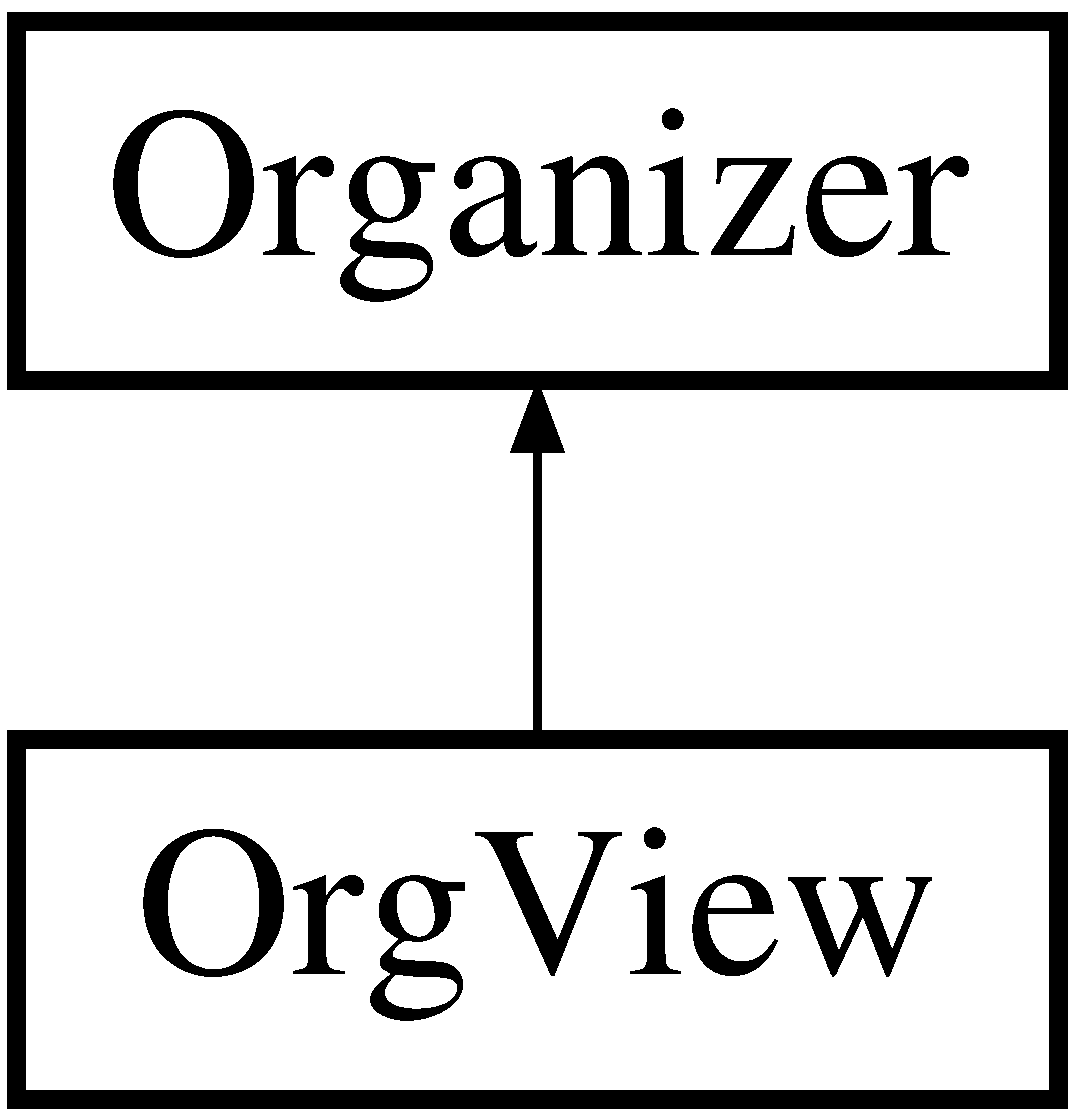
\includegraphics[height=2.000000cm]{class_organizer}
\end{center}
\end{figure}
\subsection*{Fonctions membres publiques}
\begin{DoxyCompactItemize}
\item 
{\bf Organizer} ()\label{class_organizer_a5eb7c1fc676db53752dc784136d878bd}

\begin{DoxyCompactList}\small\item\em Constructeur de la classe \doxyref{Organizer}{p.}{class_organizer}. \end{DoxyCompactList}\item 
bool {\bf create\-D\-B} () const 
\begin{DoxyCompactList}\small\item\em Créer la base de donnée sqlite3. \end{DoxyCompactList}\item 
void {\bf create\-Table} (const std\-::string \&query) const 
\begin{DoxyCompactList}\small\item\em Créer une table dans la base de donnée. \end{DoxyCompactList}\item 
void {\bf insert} (const boost\-::filesystem\-::path \&p) const 
\begin{DoxyCompactList}\small\item\em Insert un chemin dans la base de donnée. \end{DoxyCompactList}\item 
const std\-::string {\bf supprimer\-Guillemets} (const Q\-String \&Qstr)
\begin{DoxyCompactList}\small\item\em Supprime les guillemets d'une chaine de caractères. \end{DoxyCompactList}\item 
void {\bf md5} ({\bf Doublon} $\ast$d)
\begin{DoxyCompactList}\small\item\em Calcul la somme M\-D5 d'un fichier. \end{DoxyCompactList}\item 
void {\bf search\-Double} (void)\label{class_organizer_a12be02528b8c31e9b65d4df997fbe9d7}

\begin{DoxyCompactList}\small\item\em Recherche les fichiers en double. \end{DoxyCompactList}\item 
void {\bf search\-By\-Size} (const uint64\-\_\-t size)
\begin{DoxyCompactList}\small\item\em Recherche les fichiers ayant la même taille. \end{DoxyCompactList}\item 
void {\bf set\-Racine} (const std\-::string \&{\bf racine})
\begin{DoxyCompactList}\small\item\em Initialise la racine de l'arborecence. \end{DoxyCompactList}\item 
const std\-::string \& {\bf get\-Racine} () const 
\begin{DoxyCompactList}\small\item\em Récupérérer la racine de l'arborecence. \end{DoxyCompactList}\item 
void {\bf search\-Empty} ()\label{class_organizer_ae27eedbd6bdd5aeb2b42c4b90572b8b0}

\begin{DoxyCompactList}\small\item\em Recherche de dossiers vide. \end{DoxyCompactList}\item 
bool {\bf is\-Update} (const boost\-::filesystem\-::path \&p) const 
\begin{DoxyCompactList}\small\item\em Test si un dossier est à jour dans la base de données. \end{DoxyCompactList}\end{DoxyCompactItemize}
\subsection*{Attributs protégés}
\begin{DoxyCompactItemize}
\item 
std\-::multiset$<$ {\bf Doublon} $\ast$ $>$ {\bf doublon\-Size}
\item 
std\-::map$<$ {\bf M\-D5\-Key}, std\-::list\\*
$<$ boost\-::filesystem\-::path $>$ $>$ {\bf doublons}
\item 
std\-::list\\*
$<$ boost\-::filesystem\-::path $>$ {\bf empty\-Dir}
\item 
std\-::string {\bf racine}
\end{DoxyCompactItemize}


\subsection{Description détaillée}
Classe représentant l'application. 

\subsection{Documentation des fonctions membres}
\index{Organizer@{Organizer}!create\-D\-B@{create\-D\-B}}
\index{create\-D\-B@{create\-D\-B}!Organizer@{Organizer}}
\subsubsection[{create\-D\-B}]{\setlength{\rightskip}{0pt plus 5cm}bool Organizer\-::create\-D\-B (
\begin{DoxyParamCaption}
{}
\end{DoxyParamCaption}
) const}\label{class_organizer_aa0203d8ff56c2a2bc620f26b7f4acbe6}


Créer la base de donnée sqlite3. 

\begin{DoxyReturn}{Renvoie}
true si la base de donnée est ouverte false sinon 
\end{DoxyReturn}
\index{Organizer@{Organizer}!create\-Table@{create\-Table}}
\index{create\-Table@{create\-Table}!Organizer@{Organizer}}
\subsubsection[{create\-Table}]{\setlength{\rightskip}{0pt plus 5cm}void Organizer\-::create\-Table (
\begin{DoxyParamCaption}
\item[{const std\-::string \&}]{query}
\end{DoxyParamCaption}
) const}\label{class_organizer_a767df574ab8675f6c6caa72c8c0d1f77}


Créer une table dans la base de donnée. 


\begin{DoxyParams}[1]{Paramètres}
\mbox{\tt in}  & {\em query} & \-: Commande à exécuter pour la création de la table \\
\hline
\end{DoxyParams}
\index{Organizer@{Organizer}!get\-Racine@{get\-Racine}}
\index{get\-Racine@{get\-Racine}!Organizer@{Organizer}}
\subsubsection[{get\-Racine}]{\setlength{\rightskip}{0pt plus 5cm}const std\-::string\& Organizer\-::get\-Racine (
\begin{DoxyParamCaption}
{}
\end{DoxyParamCaption}
) const\hspace{0.3cm}{\ttfamily [inline]}}\label{class_organizer_ad2ba7fc945c876ab06b2fc03ab667b1c}


Récupérérer la racine de l'arborecence. 

\begin{DoxyReturn}{Renvoie}
Le chemin de la racine de l'arborecence 
\end{DoxyReturn}
\index{Organizer@{Organizer}!insert@{insert}}
\index{insert@{insert}!Organizer@{Organizer}}
\subsubsection[{insert}]{\setlength{\rightskip}{0pt plus 5cm}void Organizer\-::insert (
\begin{DoxyParamCaption}
\item[{const boost\-::filesystem\-::path \&}]{p}
\end{DoxyParamCaption}
) const}\label{class_organizer_acdbfb38595b744a703f218c56b7cdd1b}


Insert un chemin dans la base de donnée. 


\begin{DoxyParams}[1]{Paramètres}
\mbox{\tt in}  & {\em p} & \-: Chemin à insérer dans la base de donnée \\
\hline
\end{DoxyParams}
\index{Organizer@{Organizer}!is\-Update@{is\-Update}}
\index{is\-Update@{is\-Update}!Organizer@{Organizer}}
\subsubsection[{is\-Update}]{\setlength{\rightskip}{0pt plus 5cm}bool Organizer\-::is\-Update (
\begin{DoxyParamCaption}
\item[{const boost\-::filesystem\-::path \&}]{p}
\end{DoxyParamCaption}
) const}\label{class_organizer_a197fdab12212f89f461f7a46437e8ccc}


Test si un dossier est à jour dans la base de données. 


\begin{DoxyParams}[1]{Paramètres}
\mbox{\tt in}  & {\em p} & \-: Chemin d'accès à un repertoire \\
\hline
\end{DoxyParams}
\begin{DoxyReturn}{Renvoie}
true si le repertoire est à jour 
\end{DoxyReturn}
\index{Organizer@{Organizer}!md5@{md5}}
\index{md5@{md5}!Organizer@{Organizer}}
\subsubsection[{md5}]{\setlength{\rightskip}{0pt plus 5cm}void Organizer\-::md5 (
\begin{DoxyParamCaption}
\item[{{\bf Doublon} $\ast$}]{d}
\end{DoxyParamCaption}
)}\label{class_organizer_a53f3e3bc13366e77e896ff590c7da7a4}


Calcul la somme M\-D5 d'un fichier. 


\begin{DoxyParams}[1]{Paramètres}
\mbox{\tt in,out}  & {\em d} & \-: Pointeur sur un \doxyref{Doublon}{p.}{class_doublon} \\
\hline
\end{DoxyParams}
\index{Organizer@{Organizer}!search\-By\-Size@{search\-By\-Size}}
\index{search\-By\-Size@{search\-By\-Size}!Organizer@{Organizer}}
\subsubsection[{search\-By\-Size}]{\setlength{\rightskip}{0pt plus 5cm}void Organizer\-::search\-By\-Size (
\begin{DoxyParamCaption}
\item[{const uint64\-\_\-t}]{size}
\end{DoxyParamCaption}
)}\label{class_organizer_a1addfcdc39e0f88d06dec40ed4c8f3c0}


Recherche les fichiers ayant la même taille. 


\begin{DoxyParams}[1]{Paramètres}
\mbox{\tt in}  & {\em size} & \-: Taille de fichier \\
\hline
\end{DoxyParams}
\index{Organizer@{Organizer}!set\-Racine@{set\-Racine}}
\index{set\-Racine@{set\-Racine}!Organizer@{Organizer}}
\subsubsection[{set\-Racine}]{\setlength{\rightskip}{0pt plus 5cm}void Organizer\-::set\-Racine (
\begin{DoxyParamCaption}
\item[{const std\-::string \&}]{racine}
\end{DoxyParamCaption}
)\hspace{0.3cm}{\ttfamily [inline]}}\label{class_organizer_a02f870946fca1233f00da57344160dad}


Initialise la racine de l'arborecence. 


\begin{DoxyParams}[1]{Paramètres}
\mbox{\tt in}  & {\em racine} & \-: Chemin d'un repertoire \\
\hline
\end{DoxyParams}
\index{Organizer@{Organizer}!supprimer\-Guillemets@{supprimer\-Guillemets}}
\index{supprimer\-Guillemets@{supprimer\-Guillemets}!Organizer@{Organizer}}
\subsubsection[{supprimer\-Guillemets}]{\setlength{\rightskip}{0pt plus 5cm}const std\-::string Organizer\-::supprimer\-Guillemets (
\begin{DoxyParamCaption}
\item[{const Q\-String \&}]{Qstr}
\end{DoxyParamCaption}
)}\label{class_organizer_a51829ddab54c6f52acd31ee752dcf30c}


Supprime les guillemets d'une chaine de caractères. 


\begin{DoxyParams}[1]{Paramètres}
\mbox{\tt in}  & {\em Qstr} & \-: Q\-String contenant la chaine avec guillemets \\
\hline
\end{DoxyParams}
\begin{DoxyReturn}{Renvoie}
Chaîne de caractères sans guillemets 
\end{DoxyReturn}


\subsection{Documentation des données membres}
\index{Organizer@{Organizer}!doublons@{doublons}}
\index{doublons@{doublons}!Organizer@{Organizer}}
\subsubsection[{doublons}]{\setlength{\rightskip}{0pt plus 5cm}std\-::map$<${\bf M\-D5\-Key},std\-::list$<$boost\-::filesystem\-::path$>$ $>$ Organizer\-::doublons\hspace{0.3cm}{\ttfamily [protected]}}\label{class_organizer_aeeb5d47d3dc7eedccbfa4b25685e93a5}
Map contenant les chemins d'accès aux fichiers pour une clé M\-D5 donnée \index{Organizer@{Organizer}!doublon\-Size@{doublon\-Size}}
\index{doublon\-Size@{doublon\-Size}!Organizer@{Organizer}}
\subsubsection[{doublon\-Size}]{\setlength{\rightskip}{0pt plus 5cm}std\-::multiset$<${\bf Doublon}$\ast$$>$ Organizer\-::doublon\-Size\hspace{0.3cm}{\ttfamily [protected]}}\label{class_organizer_a05f940c569835259f6473fb762368e48}
Multiset contenant les pointeurs sur les doublons de tailles identiques \index{Organizer@{Organizer}!empty\-Dir@{empty\-Dir}}
\index{empty\-Dir@{empty\-Dir}!Organizer@{Organizer}}
\subsubsection[{empty\-Dir}]{\setlength{\rightskip}{0pt plus 5cm}std\-::list$<$boost\-::filesystem\-::path$>$ Organizer\-::empty\-Dir\hspace{0.3cm}{\ttfamily [protected]}}\label{class_organizer_a4b1b739d6b2ed1480f81022da9803c22}
List contenant les chemins d'accès aux dossiers vides \index{Organizer@{Organizer}!racine@{racine}}
\index{racine@{racine}!Organizer@{Organizer}}
\subsubsection[{racine}]{\setlength{\rightskip}{0pt plus 5cm}std\-::string Organizer\-::racine\hspace{0.3cm}{\ttfamily [protected]}}\label{class_organizer_a2566fc607cc0b35100704973d863b9d2}
Chemin d'accès de la racine de l'arborescence à scanner 

La documentation de cette classe a été générée à partir des fichiers suivants \-:\begin{DoxyCompactItemize}
\item 
{\bf organizer.\-h}\item 
organizer.\-cpp\end{DoxyCompactItemize}

\hypertarget{class_ui_1_1_org_view}{\section{Référence de la classe Ui\-:\-:Org\-View}
\label{class_ui_1_1_org_view}\index{Ui\-::\-Org\-View@{Ui\-::\-Org\-View}}
}
Graphe d'héritage de Ui\-:\-:Org\-View\-:\begin{figure}[H]
\begin{center}
\leavevmode
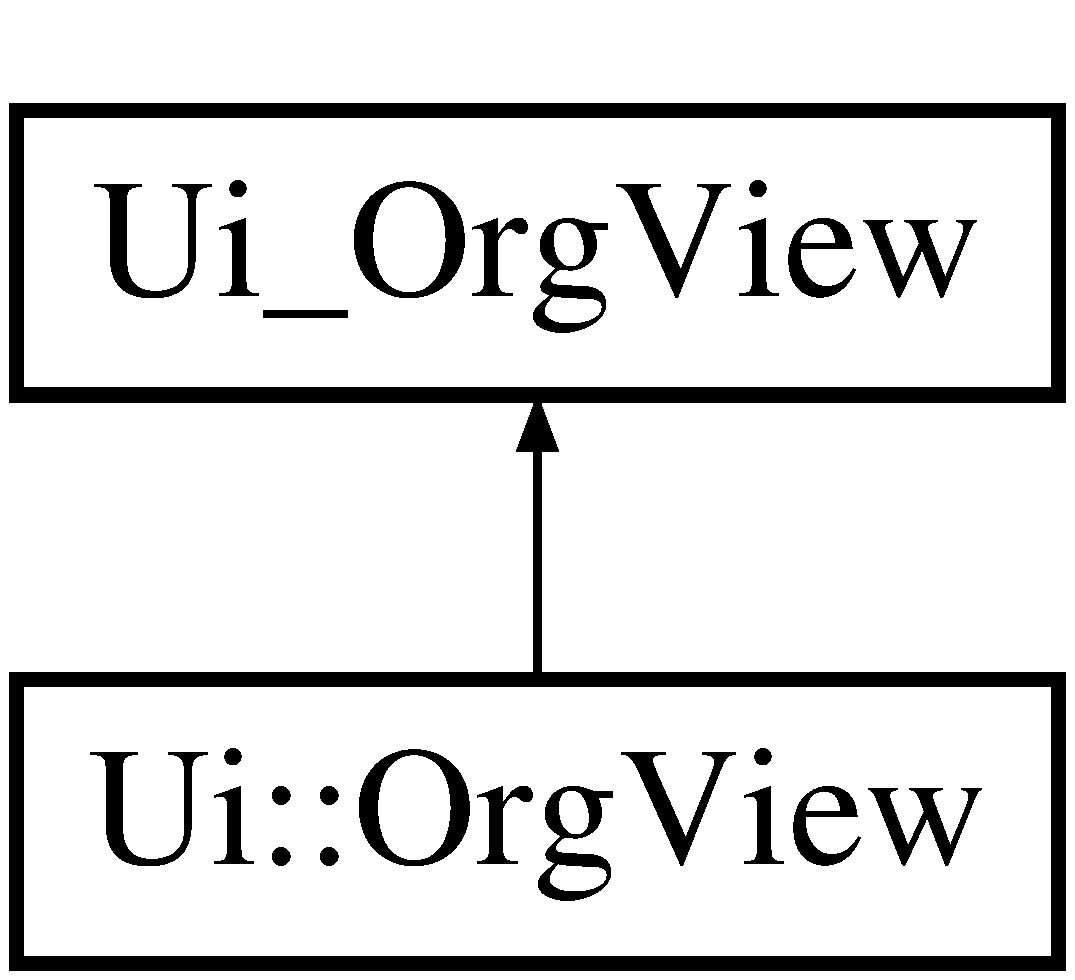
\includegraphics[height=2.000000cm]{class_ui_1_1_org_view}
\end{center}
\end{figure}
\subsection*{Additional Inherited Members}


La documentation de cette classe a été générée à partir du fichier suivant \-:\begin{DoxyCompactItemize}
\item 
ui\-\_\-orgview.\-h\end{DoxyCompactItemize}

\hypertarget{class_org_view}{\section{Référence de la classe Org\-View}
\label{class_org_view}\index{Org\-View@{Org\-View}}
}


Classe représentant l'affichage de l'application.  




{\ttfamily \#include $<$orgview.\-h$>$}

Graphe d'héritage de Org\-View\-:\begin{figure}[H]
\begin{center}
\leavevmode
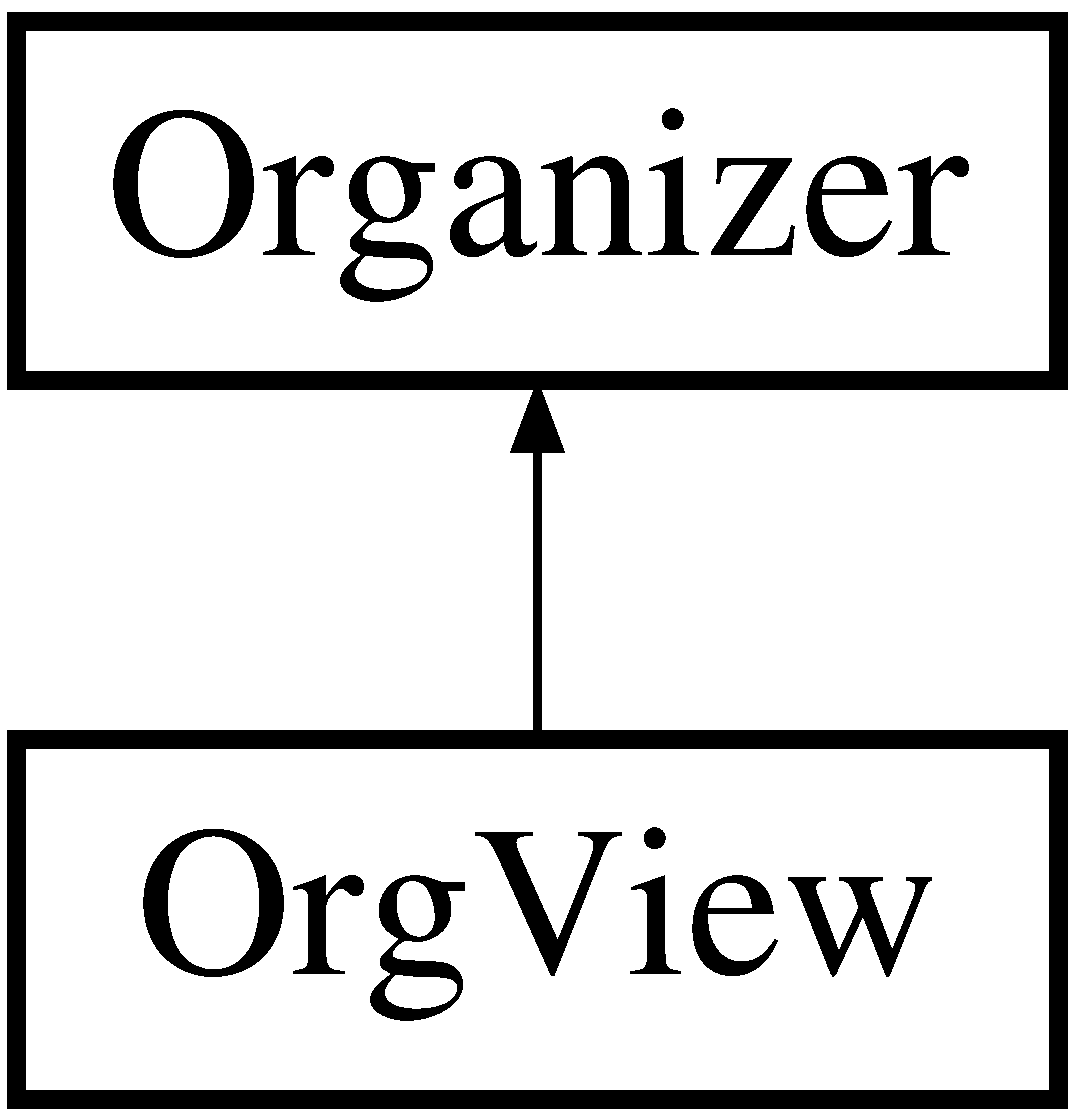
\includegraphics[height=2.000000cm]{class_org_view}
\end{center}
\end{figure}
\subsection*{Fonctions membres publiques}
\begin{DoxyCompactItemize}
\item 
\hypertarget{class_org_view_ab246039c316ff51bd026ce921f00ea55}{{\bfseries Org\-View} (Q\-Widget $\ast$parent=0)}\label{class_org_view_ab246039c316ff51bd026ce921f00ea55}

\item 
\hypertarget{class_org_view_a618029b070b1d60a49fe0696eb5be20c}{void {\bfseries start} (std\-::string argv)}\label{class_org_view_a618029b070b1d60a49fe0696eb5be20c}

\item 
\hypertarget{class_org_view_a1b58721da984696fdb169f647870291d}{void {\bfseries affiche} (const Q\-String \&s) const }\label{class_org_view_a1b58721da984696fdb169f647870291d}

\item 
\hypertarget{class_org_view_a966ec26e20729e28a7acb677f87cda75}{void {\bfseries afficher\-Doublons} ()}\label{class_org_view_a966ec26e20729e28a7acb677f87cda75}

\item 
\hypertarget{class_org_view_adc93fbb911e7a96847bbd00cc7183a42}{void {\bfseries afficher\-Empty} () const }\label{class_org_view_adc93fbb911e7a96847bbd00cc7183a42}

\item 
\hypertarget{class_org_view_a327ad745c797b4f746c79d77fc153525}{void {\bfseries set\-Status} (const std\-::string \&s) const }\label{class_org_view_a327ad745c797b4f746c79d77fc153525}

\item 
\hypertarget{class_org_view_a76cd92af0cd2b4c2b7c1de215e1b4536}{void {\bfseries delete\-File} ()}\label{class_org_view_a76cd92af0cd2b4c2b7c1de215e1b4536}

\end{DoxyCompactItemize}
\subsection*{Additional Inherited Members}


\subsection{Description détaillée}
Classe représentant l'affichage de l'application. 

La documentation de cette classe a été générée à partir des fichiers suivants \-:\begin{DoxyCompactItemize}
\item 
\hyperlink{orgview_8h}{orgview.\-h}\item 
orgview.\-cpp\end{DoxyCompactItemize}

\section{Référence de la classe Ui\-\_\-\-Org\-View}
\label{class_ui___org_view}\index{Ui\-\_\-\-Org\-View@{Ui\-\_\-\-Org\-View}}
Graphe d'héritage de Ui\-\_\-\-Org\-View\-:\begin{figure}[H]
\begin{center}
\leavevmode
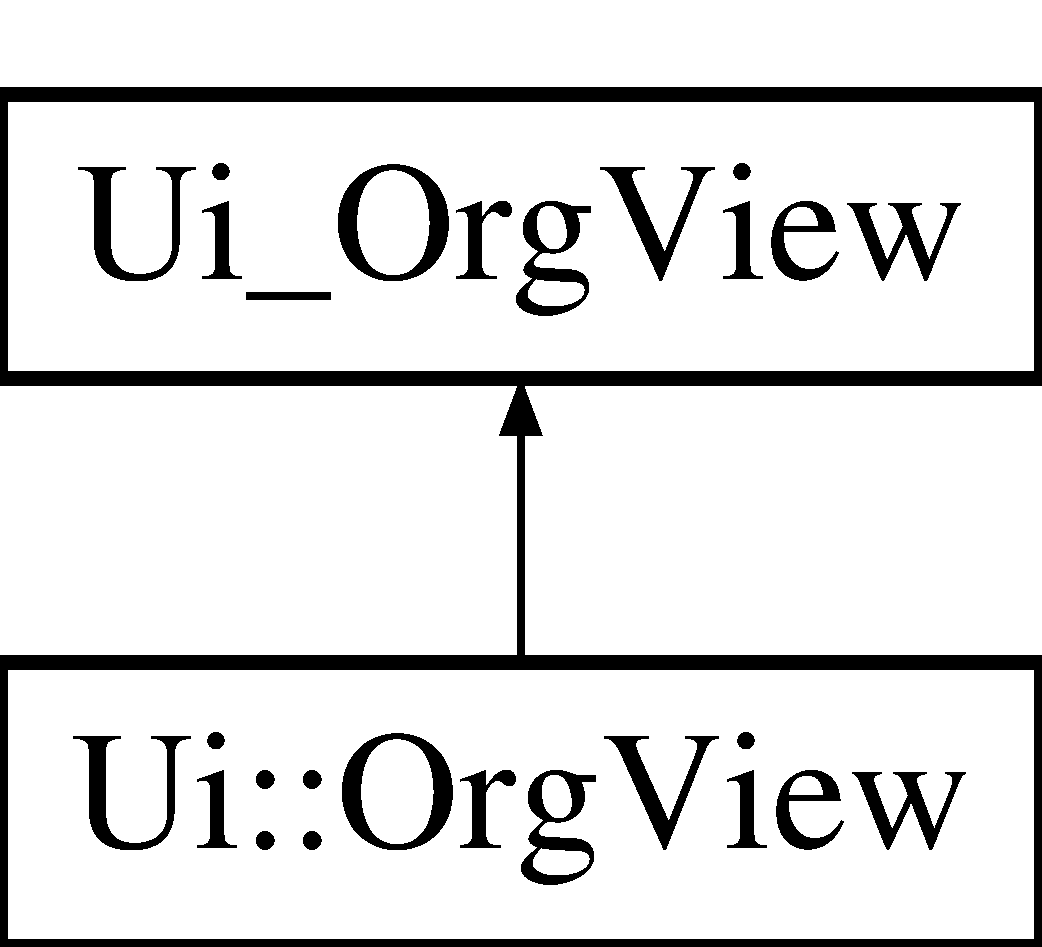
\includegraphics[height=2.000000cm]{class_ui___org_view}
\end{center}
\end{figure}
\subsection*{Fonctions membres publiques}
\begin{DoxyCompactItemize}
\item 
void {\bfseries setup\-Ui} (Q\-Main\-Window $\ast${\bf Org\-View})\label{class_ui___org_view_a19e8f7a9520c4d8aa55dcf3d2e834cc0}

\item 
void {\bfseries retranslate\-Ui} (Q\-Main\-Window $\ast${\bf Org\-View})\label{class_ui___org_view_aae8a21e7f58f6f9dd7d8c63bb37e1ee6}

\end{DoxyCompactItemize}
\subsection*{Attributs publics}
\begin{DoxyCompactItemize}
\item 
Q\-Action $\ast$ {\bfseries action\-Auteurs}\label{class_ui___org_view_a6a1ea7b9ba65e164adea9e4cf2da9a94}

\item 
Q\-Widget $\ast$ {\bfseries centralwidget}\label{class_ui___org_view_a60c22c7cae0804f412bffda4eb37fe89}

\item 
Q\-Widget $\ast$ {\bfseries widget}\label{class_ui___org_view_a500ed1d489b4d1dfebc6a81b0c61e5af}

\item 
Q\-Tab\-Widget $\ast$ {\bfseries recherche}\label{class_ui___org_view_acc72cfe0a57954b542e45813e1388662}

\item 
Q\-Widget $\ast$ {\bfseries doublons}\label{class_ui___org_view_a9bc9e46ec3a4274d2b2b9447a2340ebd}

\item 
Q\-Push\-Button $\ast$ {\bfseries search\-\_\-double}\label{class_ui___org_view_a225f3433070d7e4c89f16992bda97613}

\item 
Q\-Tree\-View $\ast$ {\bfseries tree\-View}\label{class_ui___org_view_a8fe6ded92ad2b37a338f98d09526083a}

\item 
Q\-Progress\-Bar $\ast$ {\bfseries progress\-Bar\-Double}\label{class_ui___org_view_a7e438ecee8e00a03b1d7d5c195177c54}

\item 
Q\-Push\-Button $\ast$ {\bfseries delete\-File}\label{class_ui___org_view_a63c176c0aff655c9931f59557f3ea3e1}

\item 
Q\-Widget $\ast$ {\bfseries tab}\label{class_ui___org_view_a580c7f71489da0743643d8fe14c77960}

\item 
Q\-Push\-Button $\ast$ {\bfseries search\-\_\-empty}\label{class_ui___org_view_a6ecf92571008c68476629e3ba8839ff1}

\item 
Q\-Tree\-View $\ast$ {\bfseries tree\-View\-Empty}\label{class_ui___org_view_a333b2176baad37a8063871be07b77bc9}

\item 
Q\-Progress\-Bar $\ast$ {\bfseries progress\-Bar\-Empty}\label{class_ui___org_view_a4048e44486bc30b35835dc76c3b15a58}

\item 
Q\-Push\-Button $\ast$ {\bfseries delete\-Empty}\label{class_ui___org_view_a3ef3f01b2a60312f4cda4cba06c43f23}

\item 
Q\-Text\-Browser $\ast$ {\bfseries text\-Browser}\label{class_ui___org_view_a072c0e185f24999aca89315bce02d85f}

\item 
Q\-Push\-Button $\ast$ {\bfseries start\-\_\-stop}\label{class_ui___org_view_a711bbee29b7c6ebe4e9073a0ed2e7f4a}

\item 
Q\-Tree\-View $\ast$ {\bfseries vue}\label{class_ui___org_view_ad4c16eb931a988940910273ad90ef890}

\item 
Q\-Label $\ast$ {\bfseries label}\label{class_ui___org_view_ae66a8c35e4bae47a02b1f1ca006fd480}

\item 
Q\-Label $\ast$ {\bfseries status}\label{class_ui___org_view_a3d195c0b3eda35223a31c9402dbb46cc}

\item 
Q\-Label $\ast$ {\bfseries status\-\_\-error}\label{class_ui___org_view_a810e8b7a40b0e24884c7e36ec0871497}

\item 
Q\-Menu\-Bar $\ast$ {\bfseries menubar}\label{class_ui___org_view_a25db5f5d75ec4ede06dab4539d532f2e}

\item 
Q\-Menu $\ast$ {\bfseries menu\-A\-\_\-propos}\label{class_ui___org_view_a16b200c0fe2f93152cedf3d1a1a08f2f}

\end{DoxyCompactItemize}


La documentation de cette classe a été générée à partir du fichier suivant \-:\begin{DoxyCompactItemize}
\item 
ui\-\_\-orgview.\-h\end{DoxyCompactItemize}

\chapter{Documentation des fichiers}
\hypertarget{doublon_8cpp}{\section{Référence du fichier doublon.\-cpp}
\label{doublon_8cpp}\index{doublon.\-cpp@{doublon.\-cpp}}
}


Définit les doublons.  


{\ttfamily \#include \char`\"{}doublon.\-h\char`\"{}}\\*
{\ttfamily \#include $<$string$>$}\\*


\subsection{Description détaillée}
Définit les doublons. \begin{DoxyAuthor}{Auteur}
Ducros \& Lefebvre 
\end{DoxyAuthor}
\begin{DoxyDate}{Date}
21 Janvier 2014 
\end{DoxyDate}

\section{Référence du fichier doublon.\-h}
\label{doublon_8h}\index{doublon.\-h@{doublon.\-h}}


Définit les doublons.  


{\ttfamily \#include $<$string$>$}\\*
{\ttfamily \#include \char`\"{}md5key.\-h\char`\"{}}\\*
\subsection*{Classes}
\begin{DoxyCompactItemize}
\item 
class {\bf Doublon}
\begin{DoxyCompactList}\small\item\em Classe représentant le \doxyref{Doublon}{p.}{class_doublon}. \end{DoxyCompactList}\end{DoxyCompactItemize}


\subsection{Description détaillée}
Définit les doublons. \begin{DoxyAuthor}{Auteur}
Ducros \& Lefebvre 
\end{DoxyAuthor}
\begin{DoxyDate}{Date}
21 Janvier 2014 
\end{DoxyDate}

\section{Référence du fichier md5key.\-h}
\label{md5key_8h}\index{md5key.\-h@{md5key.\-h}}


Définit les clé M\-D5 des doublons.  


{\ttfamily \#include $<$string$>$}\\*
\subsection*{Classes}
\begin{DoxyCompactItemize}
\item 
class {\bf M\-D5\-Key}
\begin{DoxyCompactList}\small\item\em Classe représentant la clé M\-D5. \end{DoxyCompactList}\end{DoxyCompactItemize}
\subsection*{Fonctions}
\begin{DoxyCompactItemize}
\item 
bool {\bf operator$<$} (const {\bf M\-D5\-Key} \&k1, const {\bf M\-D5\-Key} \&k2)
\item 
bool {\bf operator==} (const {\bf M\-D5\-Key} \&k1, const {\bf M\-D5\-Key} \&k2)
\item 
bool {\bf operator!=} (const {\bf M\-D5\-Key} \&k1, const {\bf M\-D5\-Key} \&k2)
\item 
std\-::ostream \& {\bfseries operator$<$$<$} (std\-::ostream \&os, const {\bf M\-D5\-Key})\label{md5key_8h_af1ca2bfa5d49ed749cdfa8ea935bf897}

\end{DoxyCompactItemize}


\subsection{Description détaillée}
Définit les clé M\-D5 des doublons. \begin{DoxyAuthor}{Auteur}
Ducros \& Lefebvre 
\end{DoxyAuthor}
\begin{DoxyDate}{Date}
21 Janvier 2014 
\end{DoxyDate}


\subsection{Documentation des fonctions}
\index{md5key.\-h@{md5key.\-h}!operator!=@{operator!=}}
\index{operator!=@{operator!=}!md5key.h@{md5key.\-h}}
\subsubsection[{operator!=}]{\setlength{\rightskip}{0pt plus 5cm}bool operator!= (
\begin{DoxyParamCaption}
\item[{const {\bf M\-D5\-Key} \&}]{k1, }
\item[{const {\bf M\-D5\-Key} \&}]{k2}
\end{DoxyParamCaption}
)}\label{md5key_8h_a911c35f88bf2d6ba464bb3c62d9b6b69}

\begin{DoxyParams}[1]{Paramètres}
\mbox{\tt in}  & {\em k1} & \-: \doxyref{M\-D5\-Key}{p.}{class_m_d5_key} servant à la comparaison \\
\hline
\mbox{\tt in}  & {\em k2} & \-: \doxyref{M\-D5\-Key}{p.}{class_m_d5_key} servant à la comparaison \\
\hline
\end{DoxyParams}
\begin{DoxyReturn}{Renvoie}
true si l'objet k1 n'est pas égale à l'objet k2 false sinon 
\end{DoxyReturn}
\index{md5key.\-h@{md5key.\-h}!operator$<$@{operator$<$}}
\index{operator$<$@{operator$<$}!md5key.h@{md5key.\-h}}
\subsubsection[{operator$<$}]{\setlength{\rightskip}{0pt plus 5cm}bool operator$<$ (
\begin{DoxyParamCaption}
\item[{const {\bf M\-D5\-Key} \&}]{k1, }
\item[{const {\bf M\-D5\-Key} \&}]{k2}
\end{DoxyParamCaption}
)}\label{md5key_8h_ab9ea4f1611018c7e43e9ff0a704dec58}

\begin{DoxyParams}[1]{Paramètres}
\mbox{\tt in}  & {\em k1} & \-: \doxyref{M\-D5\-Key}{p.}{class_m_d5_key} servant à la comparaison \\
\hline
\mbox{\tt in}  & {\em k2} & \-: \doxyref{M\-D5\-Key}{p.}{class_m_d5_key} servant à la comparaison \\
\hline
\end{DoxyParams}
\begin{DoxyReturn}{Renvoie}
true si l'objet k1 est plus petit que l'objet k2 false sinon 
\end{DoxyReturn}
\index{md5key.\-h@{md5key.\-h}!operator==@{operator==}}
\index{operator==@{operator==}!md5key.h@{md5key.\-h}}
\subsubsection[{operator==}]{\setlength{\rightskip}{0pt plus 5cm}bool operator== (
\begin{DoxyParamCaption}
\item[{const {\bf M\-D5\-Key} \&}]{k1, }
\item[{const {\bf M\-D5\-Key} \&}]{k2}
\end{DoxyParamCaption}
)}\label{md5key_8h_aedad54e0b5f2363c0340a9bb5a62781e}

\begin{DoxyParams}[1]{Paramètres}
\mbox{\tt in}  & {\em k1} & \-: \doxyref{M\-D5\-Key}{p.}{class_m_d5_key} servant à la comparaison \\
\hline
\mbox{\tt in}  & {\em k2} & \-: \doxyref{M\-D5\-Key}{p.}{class_m_d5_key} servant à la comparaison \\
\hline
\end{DoxyParams}
\begin{DoxyReturn}{Renvoie}
true si l'objet k1 est égale à l'objet k2 false sinon 
\end{DoxyReturn}

\section{Référence du fichier organizer.\-h}
\label{organizer_8h}\index{organizer.\-h@{organizer.\-h}}


Définit les méthodes de l'application.  


{\ttfamily \#include $<$string$>$}\\*
{\ttfamily \#include $<$stdint.\-h$>$}\\*
{\ttfamily \#include $<$boost/filesystem.\-hpp$>$}\\*
{\ttfamily \#include $<$Q\-String$>$}\\*
{\ttfamily \#include $<$set$>$}\\*
{\ttfamily \#include $<$list$>$}\\*
{\ttfamily \#include $<$map$>$}\\*
{\ttfamily \#include \char`\"{}doublon.\-h\char`\"{}}\\*
{\ttfamily \#include \char`\"{}md5key.\-h\char`\"{}}\\*
\subsection*{Classes}
\begin{DoxyCompactItemize}
\item 
class {\bf Organizer}
\begin{DoxyCompactList}\small\item\em Classe représentant l'application. \end{DoxyCompactList}\end{DoxyCompactItemize}


\subsection{Description détaillée}
Définit les méthodes de l'application. \begin{DoxyAuthor}{Auteur}
Ducros \& Lefebvre 
\end{DoxyAuthor}
\begin{DoxyDate}{Date}
21 Janvier 2014 
\end{DoxyDate}

\hypertarget{orgview_8h}{\section{Référence du fichier orgview.\-h}
\label{orgview_8h}\index{orgview.\-h@{orgview.\-h}}
}


Définit l'afichage de l'application.  


{\ttfamily \#include $<$Q\-Main\-Window$>$}\\*
{\ttfamily \#include $<$Q\-Model\-Index$>$}\\*
{\ttfamily \#include $<$Q\-Group\-Box$>$}\\*
{\ttfamily \#include $<$Q\-Item\-Selection\-Model$>$}\\*
{\ttfamily \#include \char`\"{}doublonmodel.\-h\char`\"{}}\\*
{\ttfamily \#include \char`\"{}organizer.\-h\char`\"{}}\\*
\subsection*{Classes}
\begin{DoxyCompactItemize}
\item 
class \hyperlink{class_org_view}{Org\-View}
\begin{DoxyCompactList}\small\item\em Classe représentant l'affichage de l'application. \end{DoxyCompactList}\end{DoxyCompactItemize}


\subsection{Description détaillée}
Définit l'afichage de l'application. \begin{DoxyAuthor}{Auteur}
Ducros \& Lefebvre 
\end{DoxyAuthor}
\begin{DoxyDate}{Date}
21 Janvier 2014 
\end{DoxyDate}

\printindex
\end{document}
